\clearpage

\section{Comparing the Results}
\label{sec:comparing}

In this section, we will be comparing the results obtained by both the Theoretical Analysis and the Simulation.

\subsection{Results for the System at \textit{t $<$ 0}}

In the following tables, we can observe the results already presented in previous sections now side by side, with the first
2 tables being part of the Theoretical Analysis and the 3rd one being part of the Simulation. These are displayed in this
way as a means of easier representation.

\begin{table}[htb!]
  \begin{tabular}{|l|r|}
      \hline    
      {\bf Name} & {\bf Currents [A]} \\ \hline
      I1 & 2.3690260e-04\\\hline I2 & -2.4828279e-04\\\hline I3 & -1.1380187e-05\\\hline I4 & 1.2106395e-03\\\hline I5 & -2.4828279e-04\\\hline I6 & 9.7373690e-04\\\hline I7 & 9.7373690e-04\\\hline Ib & -2.4828279e-04\\\hline Id & 9.7373690e-04\\\hline Id & 0.0000000e+00\\\hline 
  \end{tabular}
\quad
  \begin{tabular}{|l|r|}
    \hline    
    {\bf Name} & {\bf Voltages [V]} \\ \hline
    V0 & 2.2132762e-16\\\hline V1 & 5.1850419e+00\\\hline V2 & 4.9415541e+00\\\hline V3 & 4.4258319e+00\\\hline V5 & 4.9770105e+00\\\hline V6 & 5.7290070e+00\\\hline V7 & -1.9765220e+00\\\hline V8 & -2.9546889e+00\\\hline Vb & -3.5456366e-02\\\hline Vd & 7.9316995e+00\\\hline 
  \end{tabular}
\quad
  \begin{tabular}{|l|r|}
    \hline    
    {\bf Name} & {\bf Value [A or V]} \\ \hline
    @gb[i] & -2.48284e-04\\ \hline
@r1[i] & 2.369027e-04\\ \hline
@r2[i] & -2.48284e-04\\ \hline
@r3[i] & -1.13810e-05\\ \hline
@r4[i] & 1.210640e-03\\ \hline
@r5[i] & -2.48284e-04\\ \hline
@r6[i] & 9.737374e-04\\ \hline
@r7[i] & 9.737374e-04\\ \hline
v(1) & 5.185042e+00\\ \hline
v(2) & 4.941554e+00\\ \hline
v(3) & 4.425830e+00\\ \hline
v(5) & 4.977013e+00\\ \hline
v(6) & 5.729012e+00\\ \hline
v(7) & -1.97652e+00\\ \hline
v(8) & -2.95469e+00\\ \hline
v(9) & 0.000000e+00\\ \hline

  \end{tabular}
  \caption{Results for the Circuit at $t<0$}
\end{table}

The first thing the reader may notice is that, while the Theoretical Analysis results have 7 decimal places, the Simulation ones only have either 5 or 6, depending on the variable and with Cientific Notation. With this being said, all of the results of the currents are accurate until, at least, 4 decimal places with Cientific Notation, which translates into around 8 accurate decimal places in normal decimal notation. All of the results of the voltages are accurate until either the last number that appears in the Simulation results or the second to last number. Both of these observations are extremely satisfactory and lead us to conclude that our study of the circuit for $t < 0$ was successful.

\clearpage
\subsection{Results for the Initial Conditions of the System}

Now we take a look at the results of our study of the inital conditions of the circuit.

\begin{table}[htb!]
  \begin{tabular}{|l|r|}
    \hline    
    {\bf Name} & {\bf Currents [A]} \\ \hline
    Ix & 2.8670509e-03\\\hline Iy & -2.8670509e-03\\\hline I1 & 1.2662274e-18\\\hline I2 & -1.2386447e-18\\\hline I3 & -5.6774006e-20\\\hline I4 & -2.7353981e-19\\\hline I5 & -2.8670509e-03\\\hline I7 & -7.1450436e-19\\\hline Ib & -1.2386447e-18\\\hline Id & -3.0123519e-19\\\hline 
  \end{tabular}
\quad
  \begin{tabular}{|l|r|}
    \hline    
    {\bf Name} & {\bf Voltages [V]} \\ \hline
    V0 & -4.9144604e-32\\\hline V2 & -1.3014247e-15\\\hline V3 & -3.8742839e-15\\\hline V5 & -1.1245383e-15\\\hline V6 & 8.6836959e+00\\\hline V7 & 6.1145673e-16\\\hline V8 & 1.3292118e-15\\\hline Vb & -1.7688637e-16\\\hline Vd & -2.4537501e-15\\\hline 
  \end{tabular}
\quad
  \begin{tabular}{|l|r|}
    \hline    
    {\bf Name} & {\bf Value [A or V]} \\ \hline
    @gb[i] & 3.571179e-18\\ \hline
@r1[i] & -3.40748e-18\\ \hline
@r2[i] & 3.571179e-18\\ \hline
@r3[i] & 1.636985e-19\\ \hline
@r4[i] & 7.278356e-19\\ \hline
@r5[i] & -2.86705e-03\\ \hline
@r6[i] & 5.854099e-19\\ \hline
@r7[i] & 5.854099e-19\\ \hline
v(2) & 3.502198e-15\\ \hline
v(3) & 1.092010e-14\\ \hline
v(5) & 2.992175e-15\\ \hline
v(6) & 8.683696e+00\\ \hline
v(7) & -1.18828e-15\\ \hline
v(8) & -1.77636e-15\\ \hline
v(9) & 0.000000e+00\\ \hline

  \end{tabular}
  \caption{Results for the Circuit Built for finding the Inital Conditions}
\end{table}


Considering the extremely low numbers we obtained for most of the variables (e-14, e-15, ..., until e-20), these variables will be considered zero, as they are too small for the computer to actually make accurate calculations.

So, we will be only taking a look at the values for $I_5$ and $V_6$. Both of these are, once again, accurate until the last number displayed in the Simualtion results. This is, once again, an extremely satisfactory result that leaves us confident in saying these are the correct results for the Initial Conditions of the circuit.

\clearpage
\subsection{Time- and Frequency-Dependent Analysis}

Lastly, here are the graphs we obtained by analysing the system side by side, Figures \ref{fig:sbs1}, \ref{fig:sbs2} and \ref{fig:sbs3}. It is clear that all of them are identical, which leads us to conclude, once more, that the study was succsseful.

\begin{figure}[ht]
\centering
\begin{subfigure}{.5\textwidth}
  \centering
  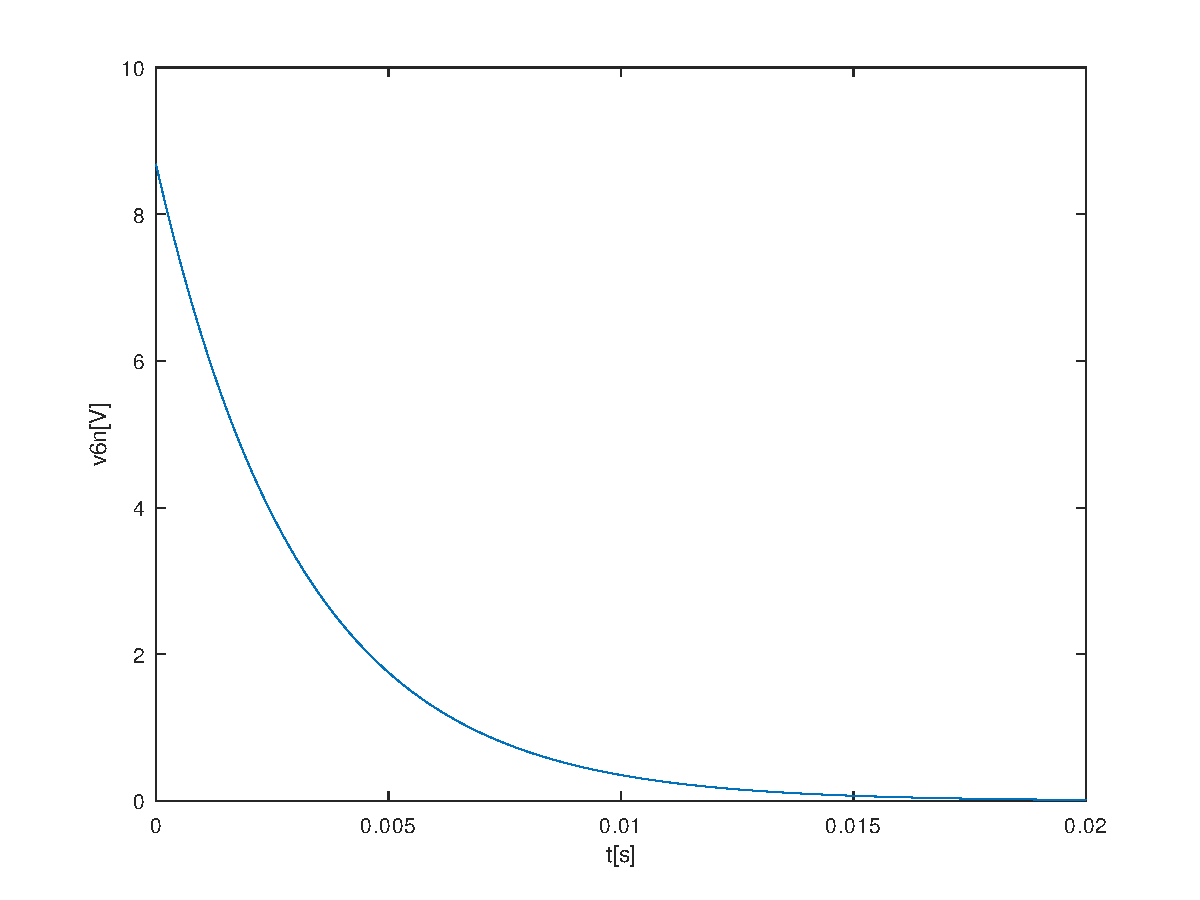
\includegraphics[width=.9\linewidth]{../mat/t2-t3.pdf}
\end{subfigure}%
\begin{subfigure}{.4\textwidth}
  \centering
  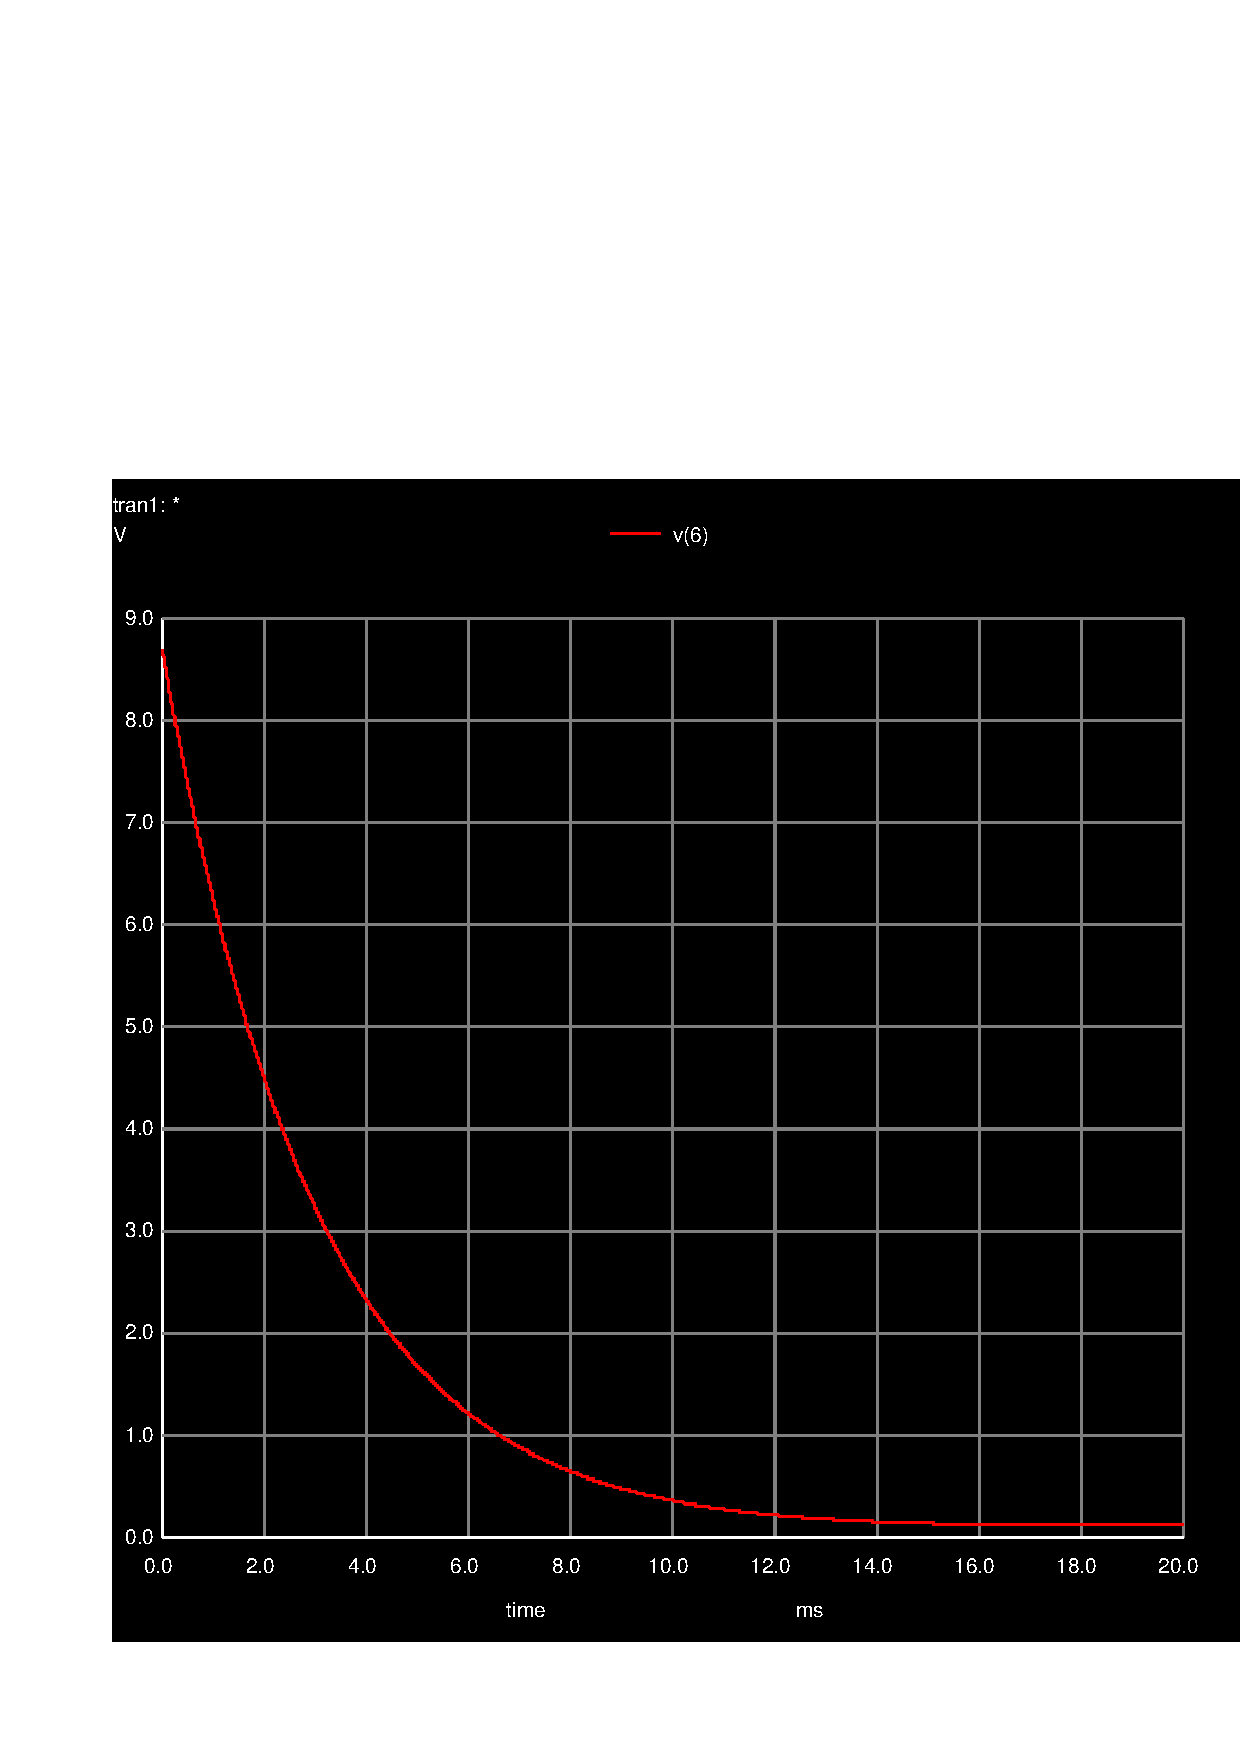
\includegraphics[width=.9\linewidth]{../sim/trans3.pdf}
\end{subfigure}
\caption{Results for f = 0Hz}
\label{fig:sbs1}
\end{figure}



\begin{figure}[ht]
\centering
\begin{subfigure}{.5\textwidth}
  \centering
  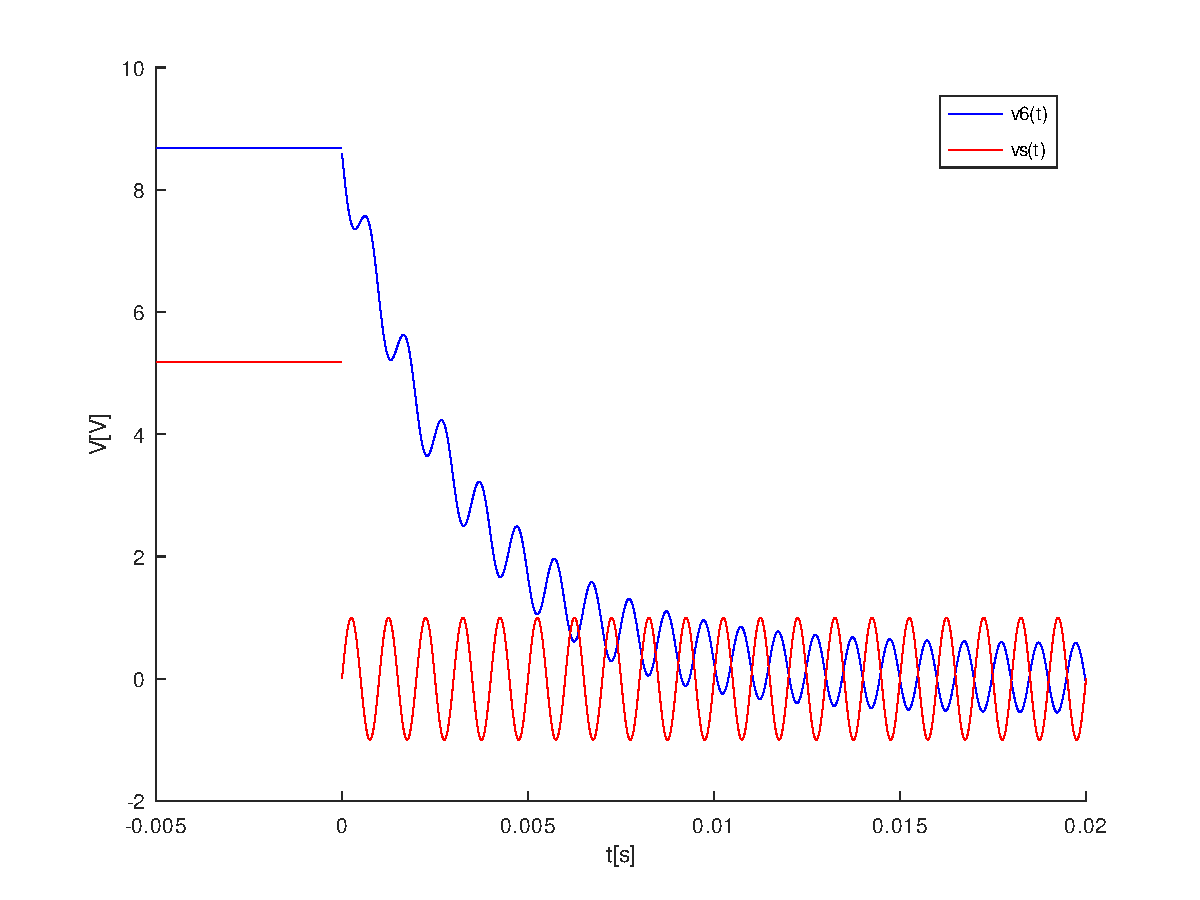
\includegraphics[width=.9\linewidth]{../mat/t2-t5.pdf}
\end{subfigure}%
\begin{subfigure}{.4\textwidth}
  \centering
  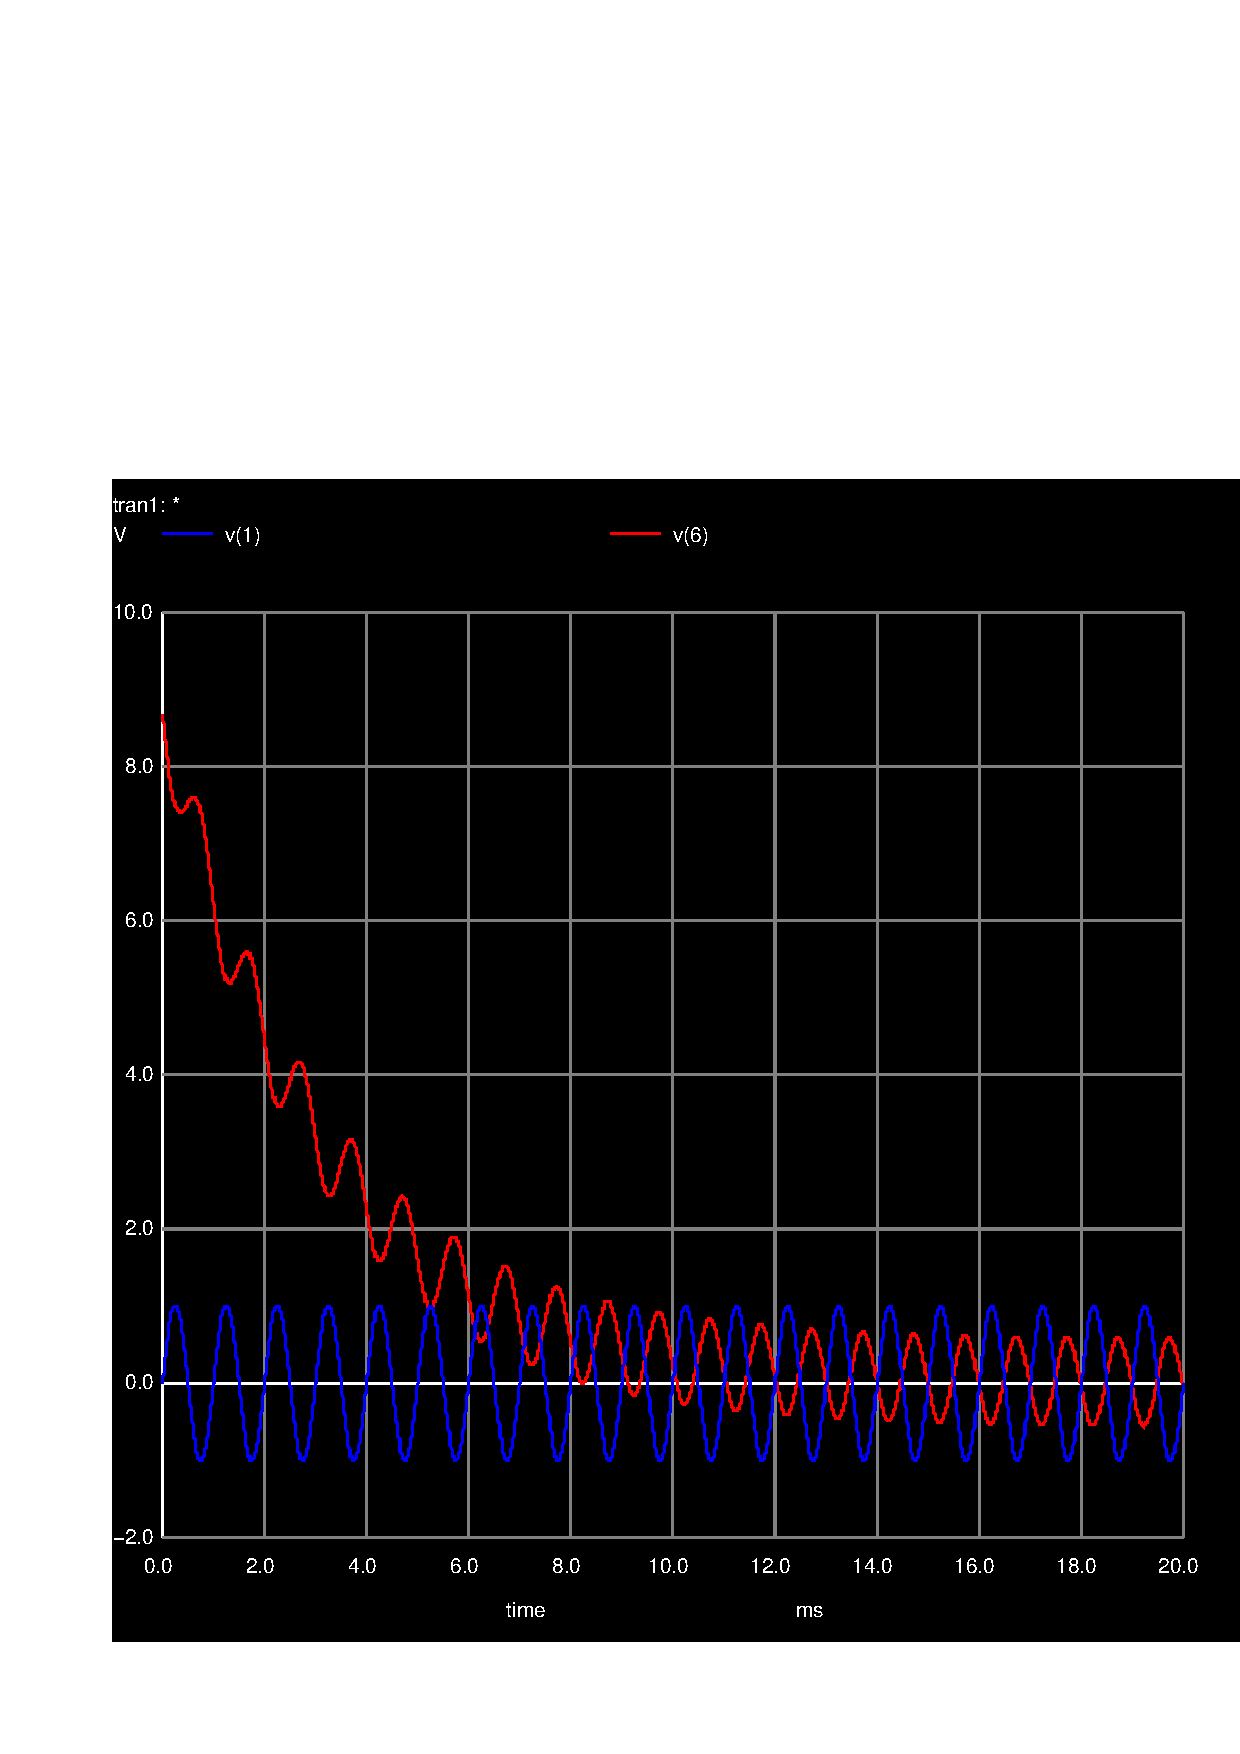
\includegraphics[width=.9\linewidth]{../sim/trans4.pdf}
\end{subfigure}
\caption{Results for f = 1kHz}
\label{fig:sbs2}
\end{figure}



\begin{figure}[ht]
\centering
\begin{subfigure}{.45\textwidth}
  \centering
  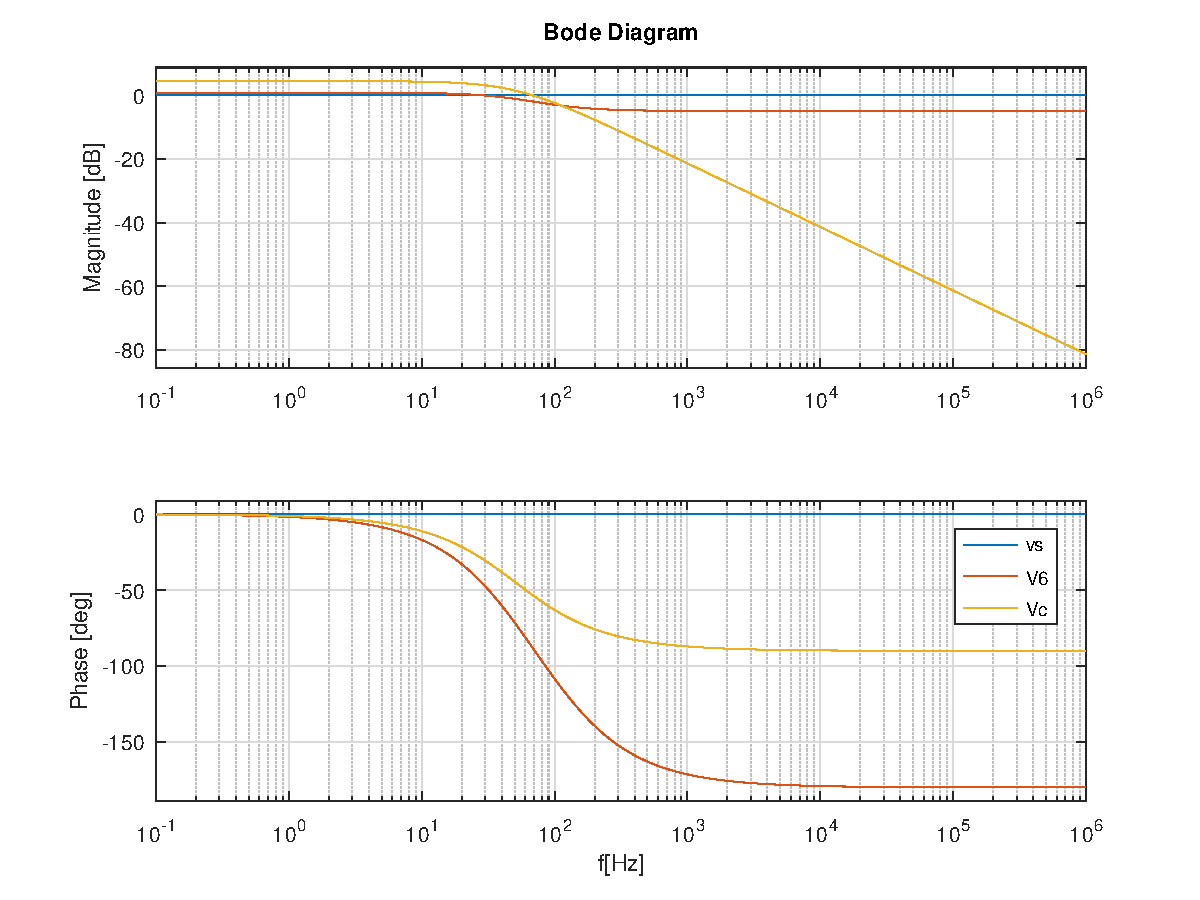
\includegraphics[width=\linewidth]{../mat/t2-t6.pdf}
\end{subfigure}%
\begin{subfigure}{.25\textwidth}
  \centering
  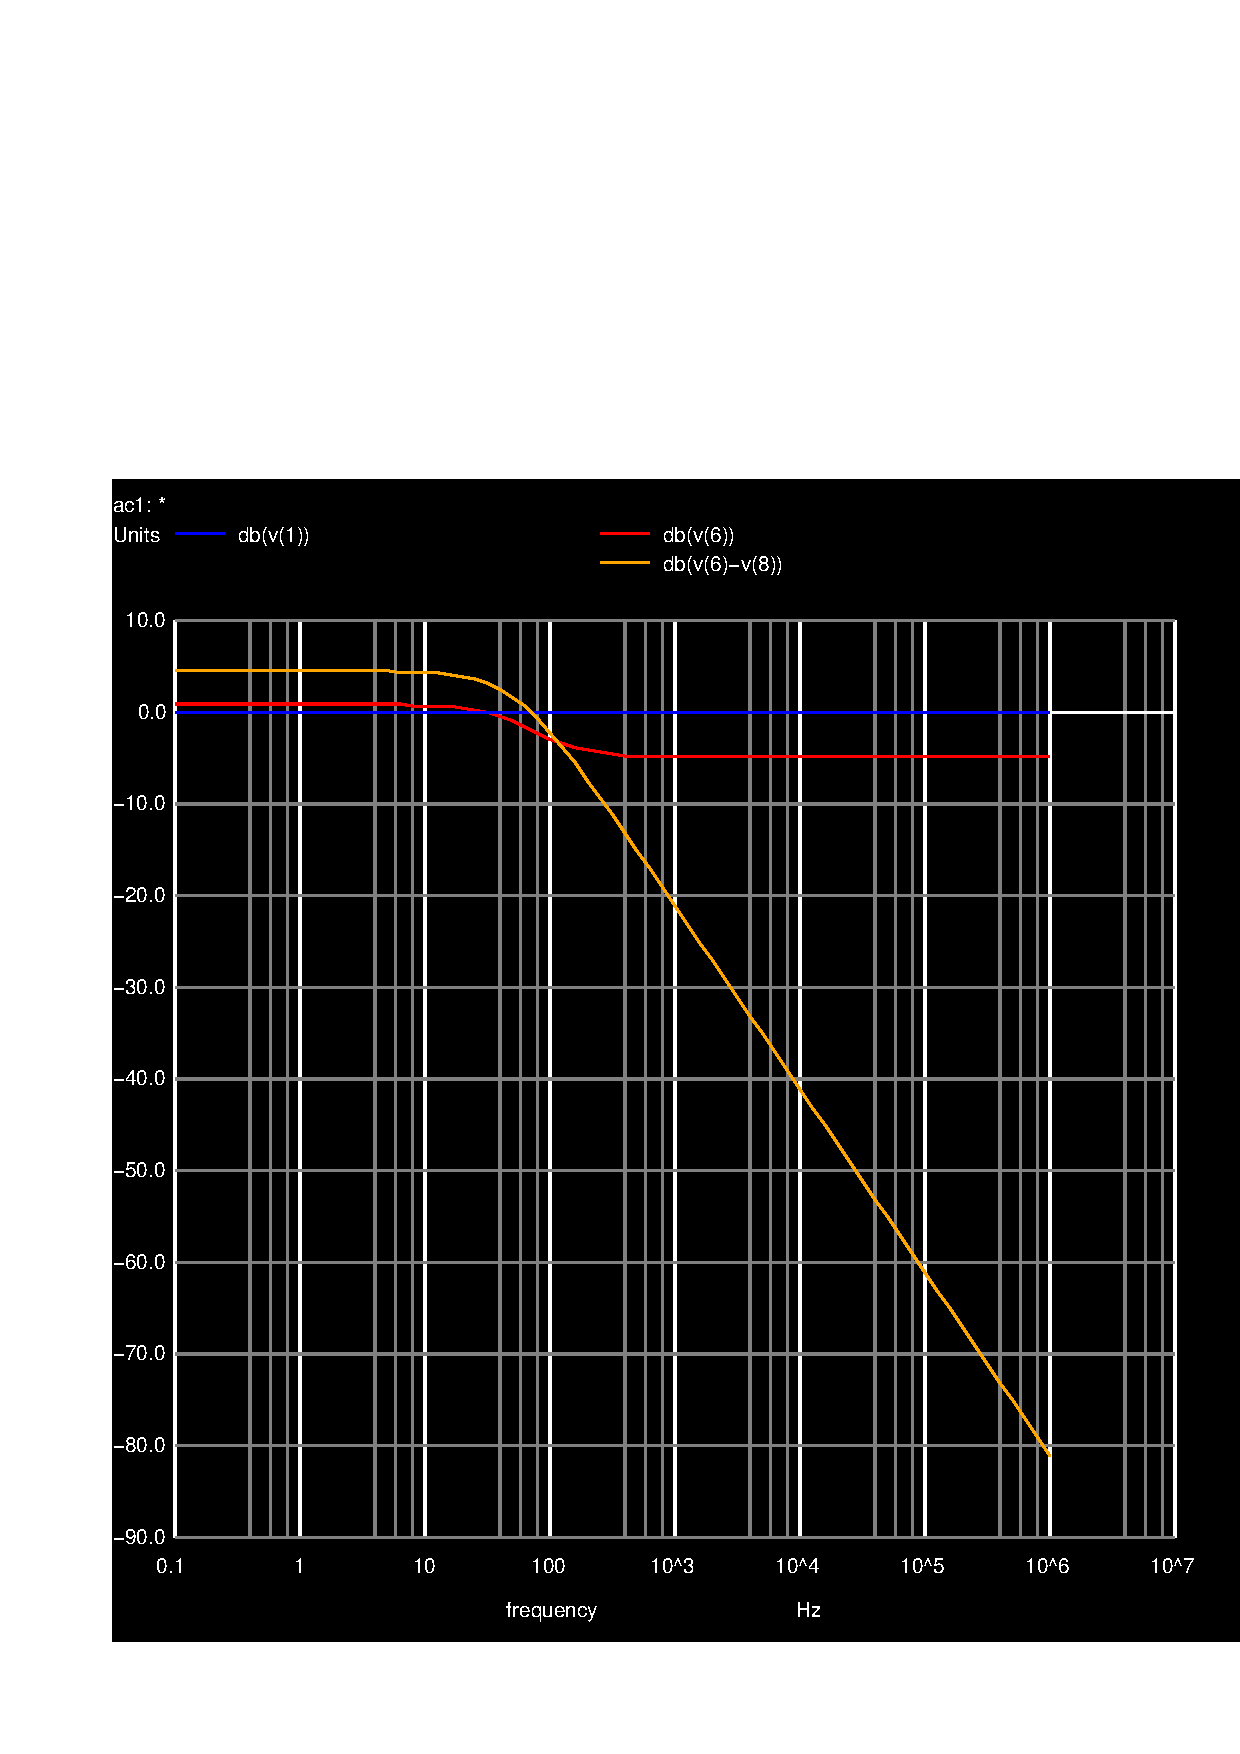
\includegraphics[width=\linewidth]{../sim/db.pdf}
\end{subfigure}
\begin{subfigure}{.25\textwidth}
  \centering
  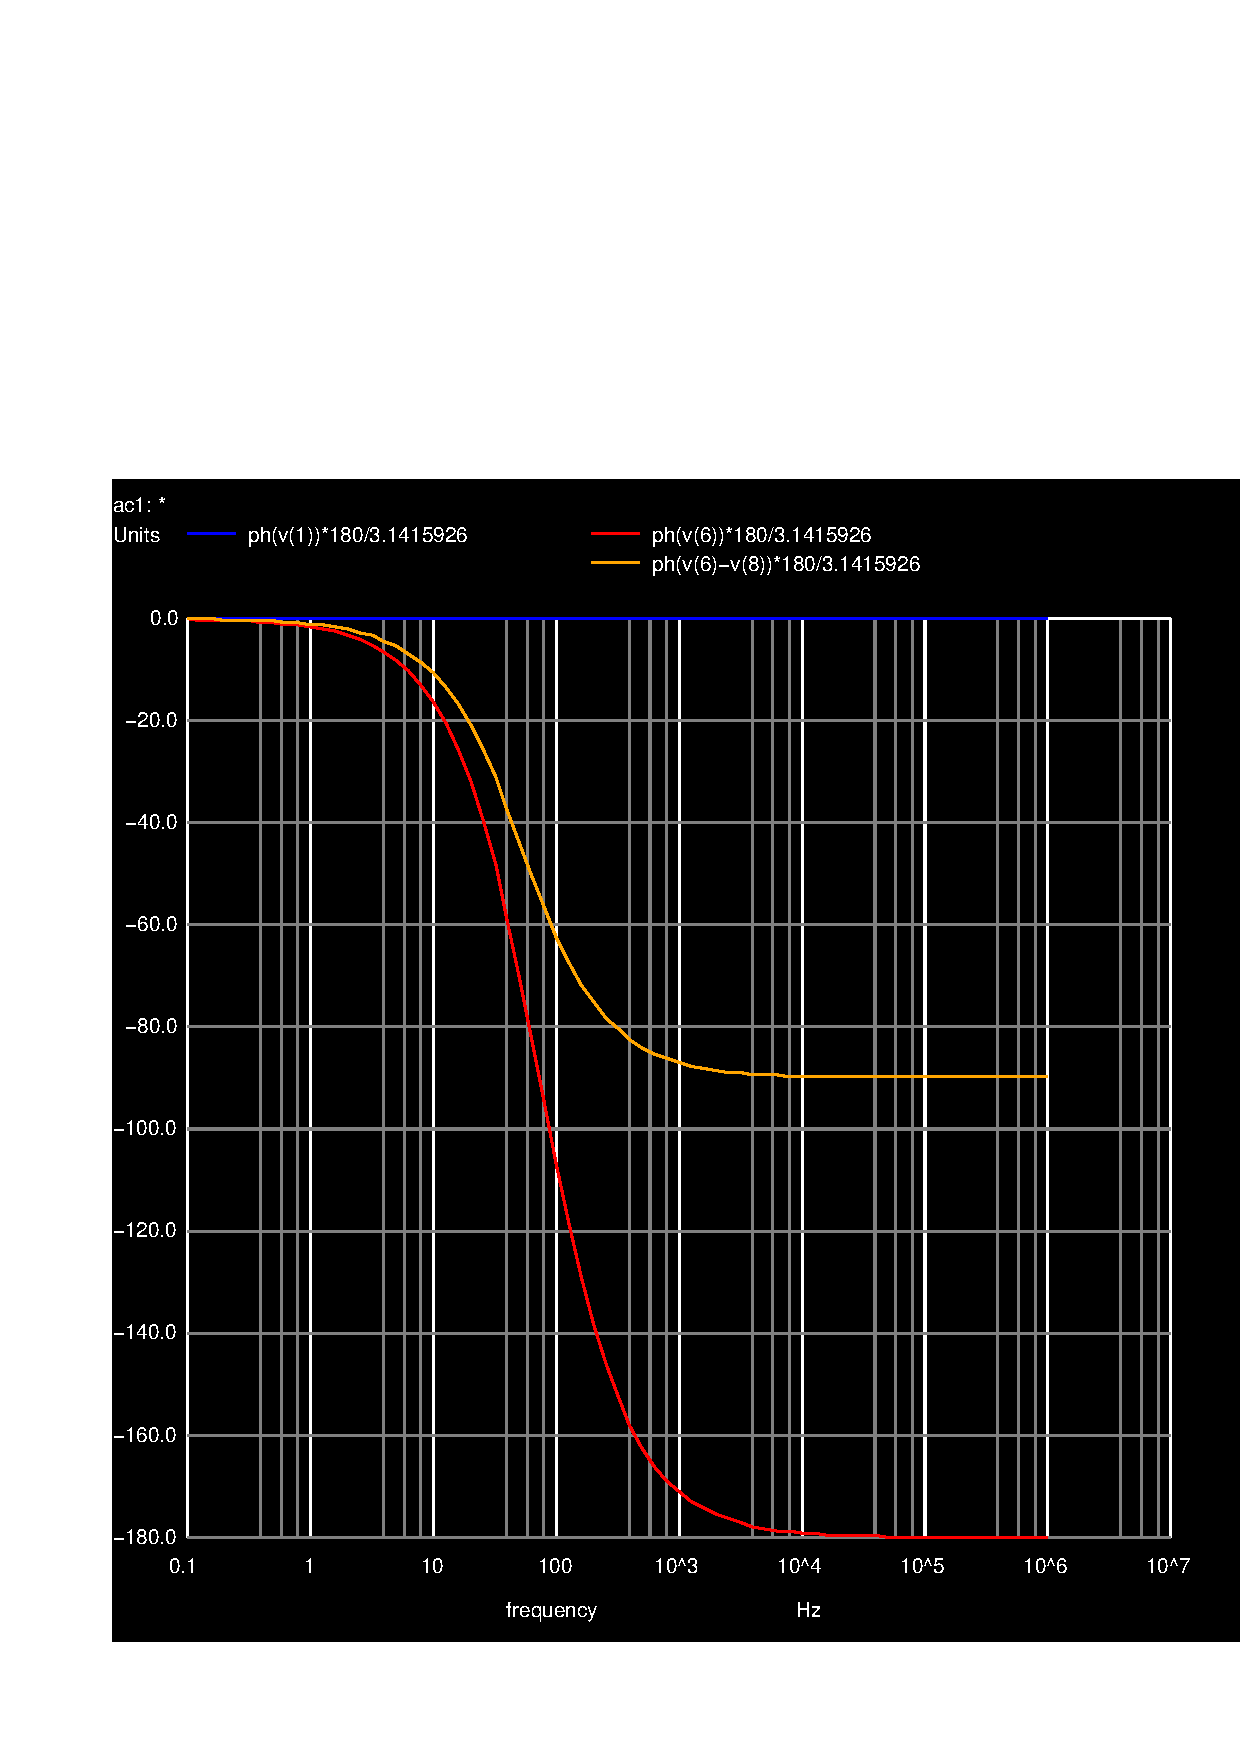
\includegraphics[width=\linewidth]{../sim/ph.pdf}
\end{subfigure}
\caption{Results for the Frequency-Dependent Analysis}
\label{fig:sbs3}
\end{figure}